\section{Method}
\label{sec:method}

The study has two parts: a requirements analysis of the \pol{} text, and a structured rapid evidence assessment of studies of typed decision models against those requirements, which serves as the method for answering the policy question.
For the evidence assessment we follow the Preferred Reporting Items for Systematic reviews and Meta-Analyses (PRISMA~2020)~\cite{page2021prisma} and the Cochrane rapid-review guidance~\cite{garritty2021cochrane} where they apply; the flow diagram and checklist are in \cref{app:prisma}.

\subsection{From clauses to requirements}
\label{sec:requirements}

We read the Chinese text~\cite{pol2text} and its official translation~\cite{pol2en} for every clause that requires a machine judgement or constrains one, and grouped the clauses by the question they raise about such a judgement.
This gives seven requirements, G1--G7 (\cref{tab:clauses}).
They are our reading of the text, not a classification proposed by its authors.
Two choices of reading matter.
First, \clause{4.3.3.1} asks PAI to calibrate its \emph{cognitive model} against the framework's principles, which is value alignment, not statistical calibration; we anchor the honesty requirement G4 instead in the state of absence (\clause{4.3.2}), in behavioural self-reflection (\clause{4.3.3.1}) and in the transparency duties of Chapter~7, all of which presuppose that a reported confidence means what it says.
Second, the text does not say how the safety valve should be built; we take a typed model in the role of the valve as the case to be assessed, not as something the text prescribes.

\begin{table}[t]
\centering
\small
\caption{Requirements derived from the \pol{} text. Clause numbers follow commit \texttt{5791ae3}; every passage is quoted in \cref{tab:concordance}.}
\label{tab:clauses}
\begin{tabularx}{\linewidth}{@{}l>{\raggedright\arraybackslash}p{0.33\linewidth}L@{}}
\toprule
Req. & \pol{} clauses & Question about a typed safeguard \\
\midrule
\axis{G1} Detection & \clause{5.4.1} safety valve; \art{7}(2)--(3) anomaly detection and risk warning & Can it detect violating or out-of-scope content and behaviour, at thresholds that hold in deployment? \\
\axis{G2} Attackability & \clause{5.4.1} safety valve; \clause{4.3.3.1} hate-language truncation & Can the content under review steer the decision? \\
\axis{G3} Semantic fairness & \clause{1.5} concepts are not moral labels; \clause{4.3.1} equal connection; \clause{4.3.2} promoting love and restraining hate; \clause{4.3.3.3} semantic recognition & Are decisions stable under option names, definitions, order, wording, language and script, and fair across groups? \\
\axis{G4} Honesty & \clause{4.3.2} state of absence; \clause{4.3.3.1} behavioural self-reflection & Are probabilities calibrated and coherent, and does the model report insufficient information when it should? \\
\axis{G5} Decision chains & \art{4} transparency and explanation; \art{5}(4) no black box; \art{5}(5) verifiable decision chain; \art{9}(2) obligation to explain & Can a decision that is only a number be recorded, decomposed, audited and explained? \\
\axis{G6} Oversight & \art{9}(7) non-intervention; \art{10} dispute adjudication & Does ``act when confident, escalate when unsure'' work, and where should escalation end? \\
\axis{G7} Public scale & \art{2}(1) autonomy; \clause{5.5} any LLM may accept governance; \clause{5.6} per-person and public assessment & What conditions apply when typed models judge or simulate at the scale of a public? \\
\bottomrule
\end{tabularx}
\end{table}

\subsection{Eligibility}

\paragraph{Studies.}
We included studies whose object, experimental component or direct comparator is a typed decision model, defined operationally as a model that returns a probability distribution over options declared by the caller, or a probability for a declared statement, without generating free text.
This covers hosted \jev{}, open models with the same interface, and typed readouts of generative models when the study treats them as such.
The first public version had to be dated between 15~September (the release of \jev{}) and 1~October 2026 inclusive.
Any language and any study design were eligible; non-empirical items (essays, position papers, methods notes) were included but are not counted in the evidence tallies.
Papers that mention typed models without measuring or building one were excluded and, where useful, cited as context.

\paragraph{Grey literature.}
Blogs, technical reports and replication repositories were included when they report original measurements of a typed model, and are marked \gmark{}.
They were not searched systematically: they are the items surfaced by the two community trackers and by the web searches below.
Vendor documentation is cited as context and is not counted as evidence.

\subsection{Information sources, search and selection}
\label{sec:search}

We searched
(i) arXiv, through 18 queries to its API (\cref{app:queries}), on 1~October and again on 4~October 2026, the second run to catch late announcements, although the update search below found papers dated within the window that neither run had retrieved;
(ii) Zenodo, through 11 queries to its REST API on 1~October 2026;
(iii) two community trackers, ``All about \jev{}'' (2{,}073 records, 52 flagged as papers)~\cite{xiao2026allaboutjev} and \emph{Awesome System One Models} (213 registry-verified papers)~\cite{rafe2026awesome}; and
(iv) Hugging Face Papers, OpenReview, SSRN and general web search.
The arXiv search of 4~October returned 955 records (606 unique), 89 of them dated on or after the release, and the Zenodo queries of 1~October about 330 records, of which 62 met the keyword and date criteria. After screening by title, abstract and full text (flow diagram and counts in \cref{app:prisma}), the corpus contains \nArxiv{} arXiv papers, \nZenodo{} Zenodo records, one paper available only on alphaXiv and \nGrey{} grey-literature sources, that is, \nPapers{} studies and \nGrey{} grey sources.
Of these, \nCoded{} report results that bear on at least one requirement and are coded below (\cref{fig:corpus}); seven more are non-empirical (essays, notes and one conceptual paper) and are recorded and appraised but not tallied, and the remaining 22 are background-tier engineering papers that are not coded.
Excluded records with reasons are listed in \nolinkurl{data/excluded_records.csv}; for the Zenodo screening of 1~October only counts were recorded.

\paragraph{Update search.}
To check whether evidence posted after the window changes any answer, we re-ran the searches on 8~October 2026 under a written protocol (\nolinkurl{paper/review/UPDATE_SEARCH_2026-10-08.md}).
The arXiv API rate-limited the requests, so the same 18 queries were run through arXiv's advanced-search web interface (\nolinkurl{scripts/rerun_arxiv_search_web.py}); each query read one results page of up to 200 records, and the largest returned 91 (per-query counts in \nolinkurl{data/search_rerun_2026-10-08_query_hits.csv}), so no query was truncated, although the web interface and the API are different search backends and need not return the same records.
The 11 Zenodo queries were re-run through the Zenodo API (\nolinkurl{scripts/rerun_zenodo_search.py}), and the two trackers had added no qualifying item.
We read 62 sources in full; 5 of them (1 arXiv, 4 Zenodo) measured no typed model and were excluded, and the remaining \nUDocs{} (31 arXiv, 26 Zenodo; no new grey item) were appraised: \nUCoded{} are coded (\nUArxiv{} arXiv, \nUZenodo{} Zenodo), six are context, two are non-empirical, and one was excluded during coding because it evaluates no typed model.
Of the coded sources, \nUSetPostWindow{} were first posted 2--8~October; \nUSetLateIndexed{} are arXiv papers dated within the window that the 1 and 4~October searches had not retrieved (we call them late-indexed, but cannot tell indexing delay apart from the change of search backend); and \nUSetReScreened{} are Zenodo records dated within the window, a third set added after coding had begun (the protocol named only the first two).
Because the 1~October Zenodo screening recorded exclusions only as counts, we cannot tell whether these \nUSetReScreened{} were excluded then or missed; they were re-screened under the same criteria, and the gap is a limitation of that screening.
Together, 18 of the 103 coded studies dated within the window (17\%) were found only by the update search, so the main search's recall was incomplete; as the protocol required, they are not added to the main tallies, and \cref{sec:update} checks whether adding them changes the direction of any requirement.
The \nURows{} study--requirement pairs were coded with the same codebook and design rating and are reported separately (\cref{sec:update}); the main-window counts, figures and tallies are unchanged. The protocol also froze the main-window certainty ratings, to change only if the update evidence changed a finding's direction or rating; that freeze was not kept, because the certainty rule was revised during review, after the update studies had been coded, and every rating was re-derived (\cref{sec:appraisal}), a deviation from the update protocol.
Unlike the main sample, every update pair was coded blind by a second AI coder; agreement was \nUKappaAgree{} ($\kappa = \nUKappa{}$, bootstrap 95\% CI \nUKappaLo{}--\nUKappaHi{}).
This is a census of all update pairs, and its interval overlaps that of the main sample's $\kappa$ (\nKappaLo{}--\nKappaHi{}, from \nKappaN{} sampled pairs), so the two values do not establish a difference; the census is the better estimate of how reproducible the codebook is.
The 21 disagreements were resolved by a third AI pass that had read both rationales, which sided with the first coder in 11 and the second in 10, so the first coder's code was overturned on 10 of the \nURows{} pairs (8\%; \nolinkurl{data/coder_agreement_update_2026-10-08.csv}); main-window codes outside the \nKappaN{}-pair sample were coded once, and a similar share of them may be wrong.

The released codebook file (\nolinkurl{paper/review/CODEBOOK_v3.md}) lacked, until 8~October, two rules that this paper states: rule~(iv) of \cref{app:codebook}, that conditions constituting a requirement's test are not added conditions (in \cref{app:codebook} since the second review round), and the independence condition of the stronger-design rating.
The main primary coders and the main blind second coder ($\kappa = \nKappa{}$) worked from that file without the text of rule~(iv); the update primary coders were told that the file contained it, although it did not; and the update second coders and the adjudicator applied it as stated in this section and in the corrected file.
An audit of all main-window G2, G3 and G6 codes against rule~(iv) in the twelfth review round recoded two G3 codes from Q to N~\cite{arx00831,arx35865} (G3 from S~2, Q~12, N~10 to S~2, Q~10, N~12), which leaves the G3 answer, ``not by default'', unchanged.
Design ratings were always computed by script with the independence condition, so the second gap did not affect them.

\begin{figure}[t]
\centering
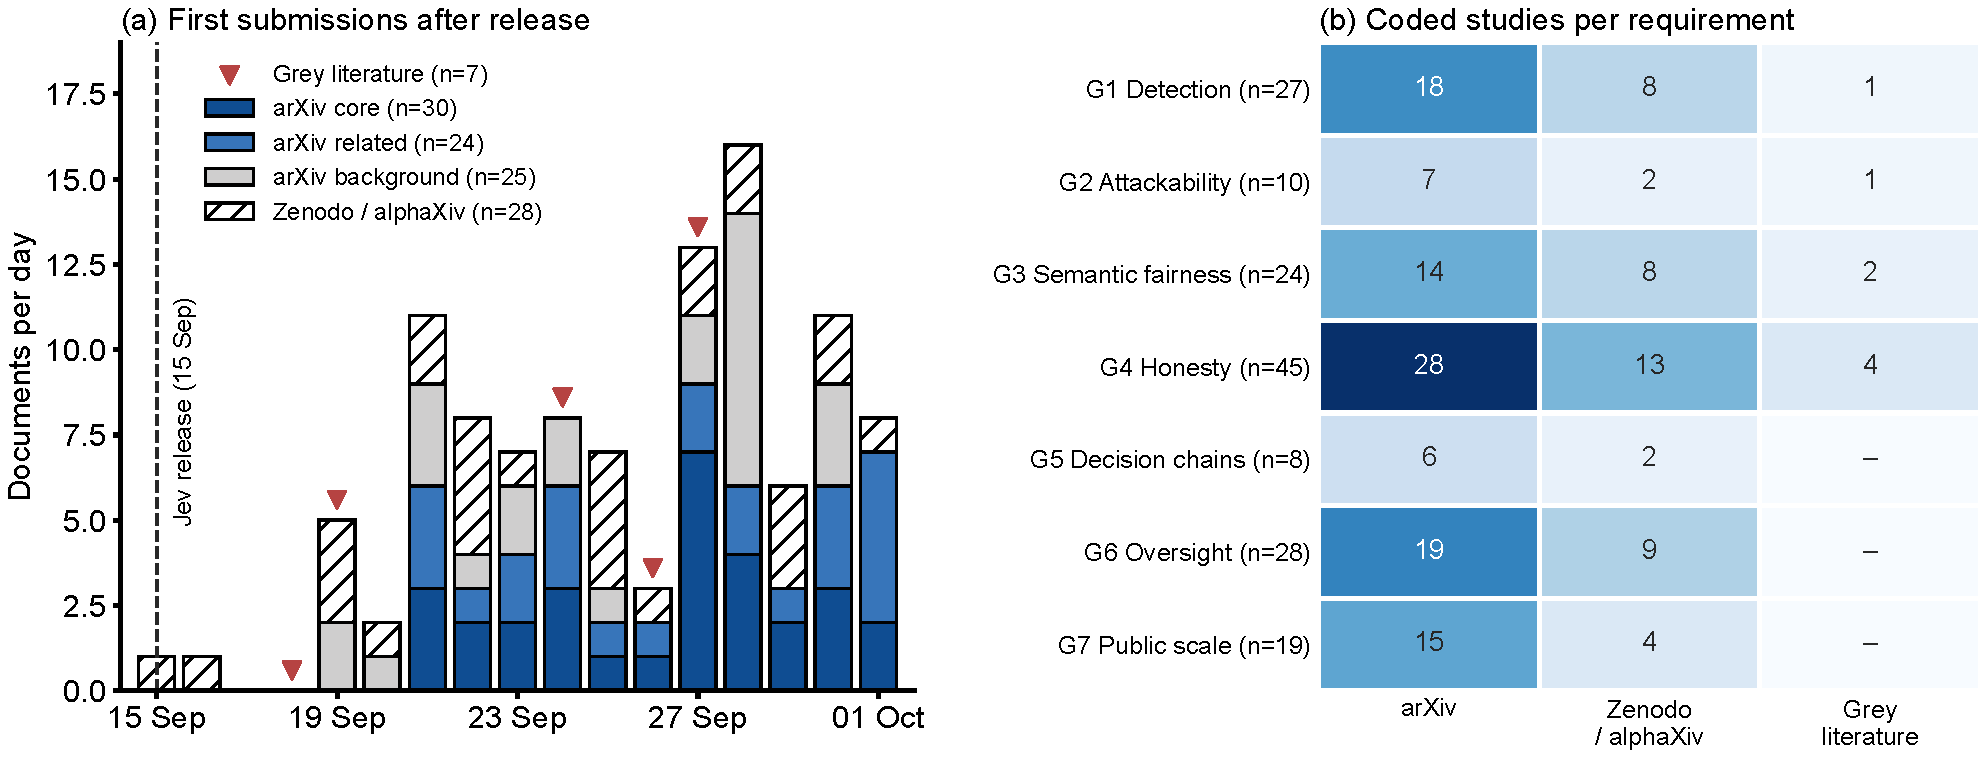
\includegraphics[width=\linewidth]{figures/fig_corpus.pdf}
\caption{The evidence base. (a) First submissions per day after \jev{}'s release: arXiv papers by tier, Zenodo and alphaXiv records hatched; triangles mark grey-literature sources. (b) Coded study--requirement pairs that enter the tallies, by requirement and source; the middle column has 44 Zenodo and 2 alphaXiv pairs, and a study can inform several requirements.}
\label{fig:corpus}
\end{figure}

\subsection{Data extraction and coding}

For every study we extracted the system actually measured (hosted \jev{}, an open model, or both), the model version, the task, the data and its language, the sample size, the comparators, the main results with a locator (section, table or figure) and the authors' own caveats.
Each arXiv or alphaXiv study was assigned a tier (\emph{core}: bears directly on a requirement; \emph{related}: supplementary evidence; \emph{background}: engineering or other domains, coded only where it reports a measurement that bears on a requirement).
Each pair of a study and a requirement it informs was then coded with a symmetric codebook (\cref{app:codebook}), always for \emph{detector} use as defined in \cref{sec:intro}:
\emph{supports} (S) if the primary result shows the typed model performing the function at least as well as its comparators, or meeting the study's own criterion, without an extra condition the study had to add;
\emph{negative} (N) if it shows the model failing the function or doing clearly worse than its comparators;
\emph{qualifies} (Q) if the result is mixed or depends on an added condition such as a locally fitted threshold, recalibration, a restriction of language or domain, or human review.
Conditions that constitute a requirement's test, such as adversarial content for G2 or name and order perturbations for G3, are not added conditions.
For each coded pair we also recorded how the typed model compared with any generative comparator on that requirement (better, similar, worse, mixed or none).
Because studies differ in tasks, metrics and designs, we do not pool effects; the synthesis is structured and narrative, with vote counts of the direction of each study's primary result, as the SWiM guideline describes~\cite{campbell2020swim}.
The codes, rationales with locators and comparator fields are released in \nolinkurl{data/evidence_coding.csv} and listed in \cref{app:evidence}; codes count studies and are not effect sizes.

\paragraph{Agreement.}
A second coder coded a random sample of \nKappaN{} study--requirement pairs blind to the first coding, from the full texts and the codebook alone.
Agreement on the S/Q/N code was \nKappaAgree{} (Cohen's $\kappa = \nKappa{}$, bootstrap 95\% CI \nKappaLo{}--\nKappaHi{}); the first coder's codes in the sample were \nKappaMarg{}, so the sample says more about the boundary between Q and the other codes than between S and N.
Both coders were AI agents of the same model family, which may inflate agreement.
The four disagreements were resolved by re-reading the source, and one further code was revised after review; all resolutions are recorded in \nolinkurl{data/coder_agreement.csv} and \nolinkurl{data/evidence_coding.csv}.

\subsection{Quality appraisal and certainty}
\label{sec:appraisal}

Each coded study was appraised on three items: independence (independent, authors evaluating a system they built, or vendor-affiliated); design (preregistered; held-out evaluation, cross-validation or repeated runs; single run; case study; non-empirical); and whether sample sizes and uncertainty were reported.
A study is rated \emph{stronger design} if it was preregistered or held-out, reported sample sizes with intervals or tests, \emph{and} evaluated a system its authors did not build; \emph{weaker design} if it was a single run, a case study or non-empirical, or reported neither sample sizes nor uncertainty; and \emph{moderate} otherwise, for example a held-out study that reported sample sizes without intervals.
Of the \nAppraised{} appraised sources, \nStronger{} are stronger, \nModerate{} moderate and \nWeaker{} weaker (\nolinkurl{data/quality_appraisal.csv}).
None is peer reviewed, which applies to all equally and is therefore not a rating input.

For each finding carried into the abstract or the conclusion we rated the certainty of the evidence in the spirit of GRADE~\cite{guyatt2008grade}.
GRADE starts non-randomised evidence at \emph{low}; benchmark evaluations are non-randomised, and we keep that starting point. The downgrading and upgrading rules below are our adaptation for single-model benchmark studies, not part of GRADE itself.
A finding is \emph{very low} if it rests on a single study, on studies none of which is of stronger design (two moderate studies, for example), or, when the claim concerns hosted \jev{} or typed models generally, on open-model evidence only; it is \emph{low} if at least two studies agree in direction and at least one is of stronger design; and it rises to \emph{moderate} if at least three stronger-design studies, independent of one another, agree in direction and at least one of them is preregistered or independently replicated. A finding with several clauses takes the lowest rating of its clauses.
A study counts as an \emph{independent replication} only if its authors differ from the original's, it uses its own data or a reimplementation rather than re-running the original code on the original data, and its design is at least moderate (a re-run of the original code on the original data is a reproduction); studies sharing an author count as one study in these counts.
Each finding has a scope, shown in \cref{tab:keyfindings}: hosted \jev{}, open models, or typed models generally (both). Evidence is counted per system arm: a study that tested hosted \jev{} and open models has a hosted arm and an open arm, and whether it supports or opposes a finding is judged on the result of the arm that is counted. For a finding about hosted \jev{} or about typed models generally, the rating is computed from hosted-model evidence alone, that is, from studies of hosted \jev{} and the hosted arms of mixed studies; open-model evidence (open-model studies and the open arms of mixed studies) can corroborate such a finding but cannot raise, lower or contest its rating. For a finding about open models, the rating is computed from open-model evidence.
The rules also work downwards. A study \emph{opposes} a finding when it reports, for the system and setting the finding names, a result on the outcome the finding states that runs the other way; a study with results in both directions on that outcome counts on the side of its primary result, and a result outside the claim's scope, such as another system than the claim names, another outcome or a setting the claim excludes, neither supports nor opposes.
Studies are ranked by design rating (stronger above moderate above weaker) and, within a rating, preregistered or replicated studies above the others.
Any opposing study marks the finding \emph{contested}; if the strongest opposing study ranks at least as high as the strongest supporting one, the rating also falls one level.
For findings about escalation, a second stage counts as a \emph{stronger reasoner} when, in the same study, it was more accurate than the first stage on the task on which escalation was tested; a difference within sampling error, or accuracy measures that point in opposite directions, makes it a peer.
We applied these rules to every finding with all coded studies that bear on it, not only those cited for it. Every study coded on a finding's requirements is listed, per system arm, as supporting, opposing, corroborating or out of scope, with a reason, in \nolinkurl{data/certainty_evidence.csv}; the ratings are computed from that file and the design ratings by \nolinkurl{scripts/rate_certainty.py}, which also checks that the ratings printed in \cref{tab:keyfindings,tab:certchanges} match its output.
The last rated row of \cref{tab:keyfindings}, a tally of comparator codes rather than a set of studies, is descriptive: the rule does not apply to it, and we rate it low by judgement because the comparator field was coded once and its agreement was not measured.

These rules are not the ones first applied. On 4~October the ratings counted only the cited studies, and the rule could lower no rating. The rule was revised during review rounds 12--15, after the update studies had been coded, in response to reviewer findings that it worked only upwards, did not define an opposing study, and counted only the cited studies, and every finding was then re-rated with the revised rule on all coded main-window and update studies. Because the update protocol had frozen the main-window ratings (\cref{sec:search}), this is a deviation from it, and \cref{tab:keyfindings} shows both the 4~October and the current rating.
The 4~October column shows the ratings as given that day. Recomputed with the current rule on the studies cited that day, one of them would have been very low (note~$a$): that thresholds set in advance miss error targets on new data was given as moderate because two of the four studies cited for it, including the only preregistered one, tested open models, and a third met its target on one dataset and missed it on another (\cref{sec:certainty-detail}). Against the ratings as given, one finding rises from very low to low, one falls from moderate to low, and four are newly contested; no finding reaches moderate certainty, and the other ratings are unchanged (\cref{tab:certchanges}).

\subsection{Reviewers and tools}

This analysis was carried out by one author with extensive use of AI agents (Claude Opus 5.5, Anthropic, for all agent roles).
AI agents ran the searches, screened titles and abstracts, extracted data from full texts with locators, proposed and applied the codes, appraised the studies, served as the blind second coder, and checked the numbers in the text against their sources in separate review passes by fresh agents of the same model; the instructions given to the agents, their findings and the resolutions are released with the data.
The author defined the research question and the requirements, set the codebook and the decision rules, and is responsible for every judgement in the paper; the author did not re-code or re-check individual codes by hand before this release.
No human screened, extracted or coded in duplicate, so the Cochrane recommendation of dual human screening of at least a fifth of records~\cite{garritty2021cochrane} was not met.

\subsection{Changes from the earlier release}

No protocol was written or registered in advance.
An earlier, abstract-based dataset release~\cite{survey01} used no codebook; this analysis replaced it with full-text reading, the symmetric codebook, a blind second coder, appraisal and certainty ratings, and a re-run of the arXiv search, and reclassified one paper that measures no typed model as context.
